% !TEX root = ../main.tex
\section{Results and Comparative Analysis}

All path costs and node counts below are deterministic, thanks to the FIFO tie-break. They come from
\code{tools/compare\_search.py} (the same code as notebook Section~4) and were re-run for this report:
costs and node counts were unchanged; only timings vary between machines.

\begin{table}[H]
\centering
\caption{Charger $\to$ each dirty cell on our \code{Environment.txt}.}
\begin{tabular}{@{}lcrrr@{}}
\toprule
Case & Path cost (UCS $=$ \astar) & Nodes UCS & Nodes \astar & \astar{} saving \\
\midrule
C$\to$D1 (3,4) & 11 & 41 & 23 & 44\,\% \\
C$\to$D2 (2,8) & 10 & 35 & 16 & 54\,\% \\
C$\to$D3 (9,9) & 18 & 72 & 59 & 18\,\% \\
C$\to$D4 (9,5) & 14 & 62 & 31 & 50\,\% \\
C$\to$D5 (9,0) & 13 & 54 & 19 & 65\,\% \\
\bottomrule
\end{tabular}
\end{table}

\begin{table}[H]
\centering
\caption{Scaling on open $n\times n$ grids: nodes expanded (UCS and \astar{} path costs equal).}
\begin{tabular}{@{}rcc@{}}
\toprule
$n$ & Corner $(0,0)\to(n{-}1,n{-}1)$: UCS / \astar & Midline left$\to$right: UCS / \astar \\
\midrule
5 & 24 / 24 & 18 / 4 \\
10 & 99 / 99 & 74 / 9 \\
20 & 399 / 399 & 299 / 19 \\
40 & 1599 / 1599 & 1199 / 39 \\
80 & 6399 / 6399 & 4799 / 79 \\
\bottomrule
\end{tabular}
\end{table}

\begin{figure}[H]
\centering
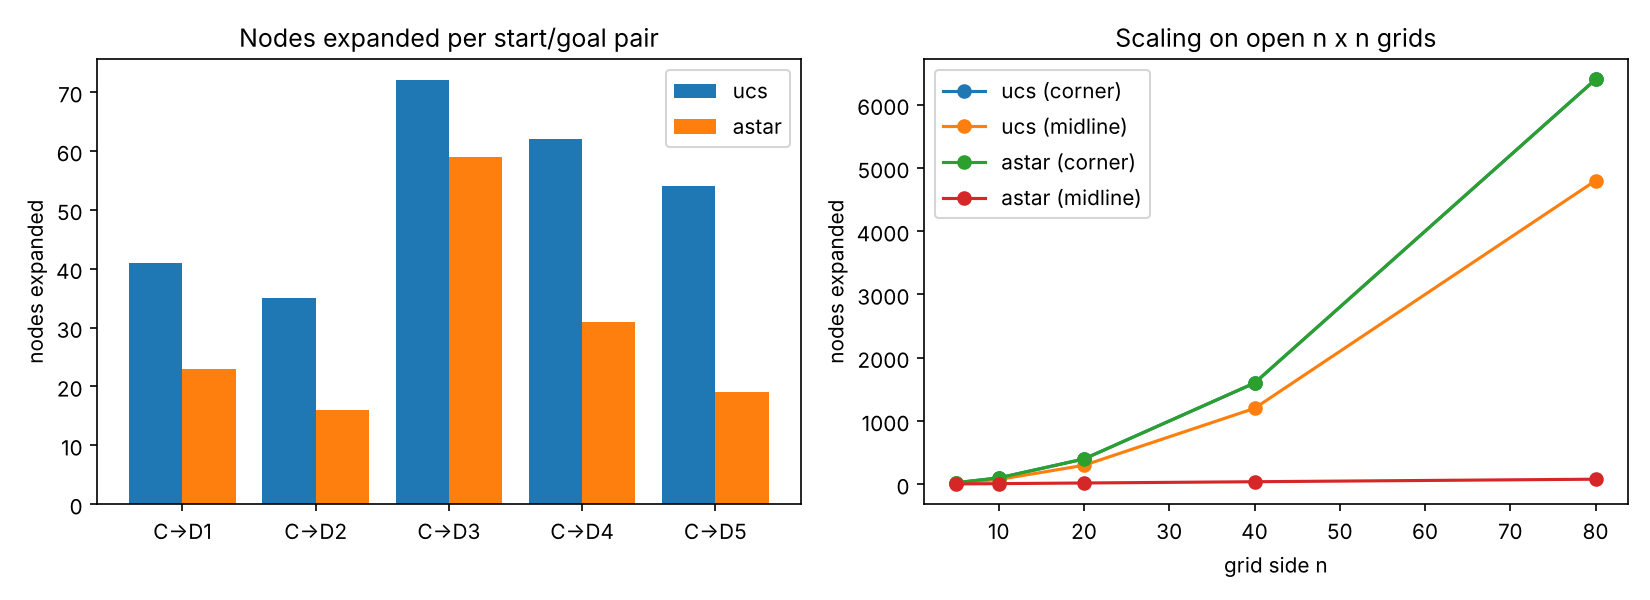
\includegraphics[width=\linewidth]{search_comparison.png}
\caption{Nodes expanded per start/goal pair on our environment (left) and scaling on open grids (right).}
\label{fig:compare}
\end{figure}

\begin{table}[H]
\centering
\caption{Full integrated runs (CSP schedule $+$ navigation, all legs including the return).}
\begin{tabular}{@{}llcrrl@{}}
\toprule
Files & Schedule & Moves $=$ cost & Nodes UCS & Nodes \astar & Status \\
\midrule
Own & D1, D2, D3, D4, D5 & 64 & 253 & 112 & success (both) \\
Sample & D2, D1, D3, D4 & 34 & 139 & 52 & success (both) \\
Error & D1, D2, D3, D4, D5 & 46 (stopped) & 259 & 156 & failure: D5 unreachable \\
\bottomrule
\end{tabular}
\end{table}

\textbf{Discussion.}
\begin{itemize}
  \item \emph{Path cost.} UCS and \astar{} found paths of equal cost in every run, as expected: both
    are optimal (Manhattan distance is admissible and consistent). The \emph{paths} can still differ
    when several optimal paths exist. On our grid, the leg C$\to$D1 goes via (4,0),(5,0) under UCS
    and via (3,1),(4,1) under \astar; both have cost 11 (Figures~\ref{fig:run1-ucs} and~\ref{fig:run1-astar}).
  \item \emph{Nodes expanded.} On our environment, \astar{} expanded 18--65\,\% fewer nodes per pair,
    and 56\,\% fewer over the whole integrated route (112 vs 253). The smallest gain is C$\to$D3: the
    walls force a long detour, so Manhattan distance underestimates more and many cells share the
    lowest $f$.
  \item \emph{Geometry decides the benefit.} On an open grid from corner to corner, every cell in the
    bounding box has the same $f = 2(n-1)$. The heuristic then cannot rule anything out, and \astar{}
    ties UCS at $n^2-1$ nodes. Along the midline only one shortest path exists, so \astar{} expands
    exactly $n-1$ nodes (linear), while UCS grows a ``diamond'' of equal $g$ around the start (about
    $0.75\,n^2$). At $80\times80$ this is 79 versus 4799.
  \item \emph{Time and memory.} Per node, \astar{} does slightly more work (one heuristic call per
    push), which is visible where both expand the same nodes. Whenever \astar{} expands fewer nodes,
    it also wins on time and frontier size.
  \item \emph{Unreachable goal.} Both algorithms expanded all 69 cells reachable from D4 in the error
    grid before reporting ``no path''. With no path to find, the heuristic gives no saving.
\end{itemize}
